\documentclass[letterpaper,12pt]{scrartcl}
\usepackage{amsmath,amsthm,amssymb,graphicx,setspace,natbib,dcolumn,float,booktabs,bm,footmisc,url,longtable,lscape,titling,hyperref,newtxtext}
\usepackage[top=1in,bottom=1in,outer=1in,inner=1in]{geometry}
\usepackage[justification=raggedright,labelsep=period,labelfont=bf,singlelinecheck=off]{caption}
\usepackage[normalem]{ulem}
\urlstyle{same}
\bibpunct[, ]{(}{)}{;}{a}{}{,}
\newcolumntype{a}{D{.}{.}{0}}
\newcolumntype{b}{D{.}{.}{2}}
\newcolumntype{d}{D{.}{.}{3}}
\newcolumntype{,}{D{,}{,}{-1}}

% \setlength{\footnotesep}{\baselineskip}
% \let\footnotesize\normalsize
% \let\oldfootnote\footnote
% \renewcommand\footnote[1]{\oldfootnote{\hspace{2mm}#1}}

\renewcommand{\bibname}{References}

% == Cross Referencing Different Docs
\usepackage{xr}
\externaldocument{appendix_JCR}

% == control space within footnote
\usepackage{setspace}
\renewcommand{\footnotelayout}{\setstretch{1}}
\setlength{\footnotemargin}{4mm}

% the following script is needed to reference appendix in the main text when using overleaf
\makeatletter
\newcommand*{\addFileDependency}[1]{% argument=file name and extension
\typeout{(#1)}% latexmk will find this if $recorder=0
% however, in that case, it will ignore #1 if it is a .aux or
% .pdf file etc and it exists! If it doesn't exist, it will appear
% in the list of dependents regardless)
%
% Write the following if you want it to appear in \listfiles
% --- although not really necessary and latexmk doesn't use this
%
\@addtofilelist{#1}
%
% latexmk will find this message if #1 doesn't exist (yet)
\IfFileExists{#1}{}{\typeout{No file #1.}}
}\makeatother

\newcommand*{\myexternaldocument}[1]{%
\externaldocument{#1}%
\addFileDependency{#1.tex}%
\addFileDependency{#1.aux}%
}

% change this to 0 to show author names
\newcommand{\blind}{1}
% change this to 0 to show tables and figures
% which are excluded from POQ word count
\newcommand{\counting}{0}

\preauthor{}
\postauthor{}
\predate{}
\postdate{}

\title{
  \textbf{\textsf{\LARGE The Rally Effect Reexamined:\linebreak New Insights from Weekly Polling Data in Japan}}\if0\blind\thanks{\hspace{3mm}Earlier versions of this study were presented at the 2018 annual meeting of the Japanese Association of Electoral Studies and workshops at Gakushuin University, University of Tokyo, and Keio University. We thank the participants of these meetings for their helpful suggestions. We also thank Yukio Maeda for providing some of the data from Kyodo News. Moreover, We are grateful to Haruka Gumizawa, Takaya Kanno, Ayano Shimbo, Rinoa Suda, and Momoka Ueda for their research assistance. This work was supported by the Japan Society for the Promotion of Science KAKENHI Grant Number~JP21K13233.} \fi
}
\author{
  \if0\blind
  \hspace{1.5in}
  Hirofumi Miwa\thanks{Professor, Faculty of Law, Gakushuin University,
  Tokyo, Japan. URL: \href{https://sites.google.com/site/miwahirofumi/en}{https://sites.google.com/site/miwahirofumi/en}}
  \hspace{.7in}
  Tomoya Sasaki\thanks{Ph.D. Candidate, Department of
  Political Science, Massachusetts Institute of Technology,
  Cambridge, MA, 02139. Email:
  \href{mailto:tomoyas@mit.edu}{tomoyas@mit.edu},
  URL: \href{https://tomoya-sasaki.github.io/}{https://tomoya-sasaki.github.io/}}
  % \hspace{.7in}
  \fi
}
\date{}

\begin{document}

\maketitle
\thispagestyle{empty}
\setcounter{page}{0}
\parindent=20pt
%\defcitealias{CSIS2023}{CSIS}
%\defcitealias{PCIA2023}{PCIA}
%\defcitealias{START2022}{START}

\vspace{-5mm}
\begin{abstract}
\noindent
This article empirically examines the ``rally 'round the flag'' phenomenon, considering the types of international phenomena that trigger the effect and the duration of the effect. Based on novel weekly polling data in Japan from 2001 to 2023, we study the rally effect for various international events and the duration of this effect. We employ a dynamic linear model to examine how military threats from North Korea and terrorism with varying severity affect Cabinet approval ratings in Japan. Our findings reveal the effect heterogeneity based on the type of event, where more severe threats like nuclear tests and terrorism targeting Japanese citizens increase government popularity, while less severe events do not. Furthermore, we find that the influence of Japanese-targeted terrorism diminishes within a week, which suggests the temporary nature of the rally effect for certain events. These insights contribute to the extensive empirical research on the rally effect. (148 words)
\end{abstract}

\bigskip
\bigskip
\noindent \textbf{Keywords}: rally 'round the flag effect, government popularity, military threat, terrorism, pooling the polls, Japan

\newpage
% \renewcommand{\footnotelayout}{\doublespacing}
\doublespacing

\noindent
The ``rally 'round the flag'' effect, a short-term increase in support for the government prompted by international conflict or similar events, is a widely discussed phenomenon in international relations and public opinion literature. Initially introduced by \citet{Mueller1970APSR}, this concept has been empirically examined in various contexts \citep[e.g.,][]{Oneal1995PolitBehav,Baker2001JCR,Chapman2004JCR,Lai2005ISQ,seo2023}, and is also acknowledged by practitioners. For instance, some media outlets have suggested that former President Trump's decision to attack Syria in April 2017 was an attempt to exploit the effect.\footnote{\url{https://www.nytimes.com/2017/04/10/opinion/war-as-political-weapon.html} (accessed June 18, 2024).}

Although rich empirical evidence has been documented, two major aspects of Mueller's initial description of the phenomena---``international crises and \textit{similar phenomena} will give a President a \textit{short-term boost} in popularity'' \citep[][p.~20; emphasis added by authors]{Mueller1970APSR}---remain underexplored. First, existing empirical studies on the rally effect have focused on international crises with military involvement and overlooked other international incidents, mostly because scholars have primarily investigated the phenomena in the U.S. context. Second, due to data limitations, expecially on the frequency, the empirical examination of the rally effect has been challenging. Moreover, previous studies tend to suffer from the endogeneity problem in that increased military tensions may be driven by a leader's diversionary strategies to stem the (expected) decline in government approval.


% Particularly, (1) Which types of international phenomena can trigger the effect? (2) How long does the effect last? Regarding the first question, existing empirical studies on the rally effect have focused on international crises with military involvement and overlooked other international incidents, mostly because scholars have primarily investigated the phenomena in the U.S. context. The second question has often been neglected due to data limitations, though it is a key observable implication of the rally effect. Moreover, previous studies tend to suffer from the endogeneity problem in that increased military tensions may be driven by a leader's diversionary strategies to stem the (expected) decline in government approval.

We address these challenges and uncover the aforementioned observable implications by analyzing the impact of various international incidents on Japan's government approval rates with the weekly polling data. Japan, with its ``Peace'' Constitution, is ideally suited for this study, as it is unlikely to initiate provocations, allowing us to view these incidents as external shocks. Therefore, we can interpret these incidents as pure external threats rather than reactions to deliberate provocations intended to divert public attention from domestic discontent or subsequent military actions. This enables us to identify the rally effect as a direct public response to international incidents, unaffected by potential effects from diversionary foreign policy.

As the explanatory variables, we choose two external security threats as incidents with different levels of intensity that potentially alter public attitudes towards the Japanese government: North Korea's military provocations---nuclear and missile tests---and terrorism abroad---Japanese-targeted and otherwise. Among these incidents, we examine the effect for different levels of severity: nuclear tests and Japanese-targeted terrorism are more salient than missile tests and other terrorism. Using these threats as rally-inducing events is a hard test for detecting the rally effect since their impact on society may be much weaker than those of international crises in which a country is directly, perhaps militarily, involved.

For the outcome variable, we compile novel weekly Cabinet approval polling data constructed from a total of 1,975 opinion polls conducted by 12 polling firms on weekends between 2001 and 2023. This fine-grained data allows us to evaluate the duration of the rally effect at a daily level by calculating the date difference between the event and the timing of polls. We analyze this fine-grained polling data with the ``pooling the polls'' method proposed by \citet{Jackman2005AustJPolitSci}.

Our empirical results show heterogeneity across different types of events in terms of effect sizes. In particular, we find that two more severe events, nuclear tests by North Korea and Japanese-targeted terrorism, have positive effects on Cabinet approval with high certainty, whereas the effects of the other two relatively minor events, missile tests and other terrorism, are smaller or negligible. These results indicate that international incidents with massive impacts, such as highly provocative military activities by North Korea or terrorism targeting their nationals, can generate the rally effect in the absence of any military reactions by the targeted government.

Furthermore, we find heterogeneity in the duration of the effects. The effect of Japanese-targeted terrorism attenuates as the elapsed time between the polling date and the event gets larger. In fact, the effect size decreases by around 5 percentage points within a week. However, the effects of other events do not change in a substantively meaningful manner over time. These results suggest that the rally effect can be extremely short for some less impactful events, which can only be captured by examining this kind of fine-grained time-series polling data.

We make the following three contributions. First, our study reveals key observable implications of the rally effect with a novel empirical setup, which examines its duration in response to various international events. Existing studies have not systematically explored how fast the effect may decay, even though ``a short-term boost'' is key to the concept. The main reason has been limited data availability, since prior works have mostly used polling data collected either monthly \citep{marra1990,Parker1995POQ,Baker2001JCR,Lai2005ISQ} or less frequently \citep{lee1977,Kam2008POQ}. We overcome this gap with weekly polling data and provide evidence of the duration of the effect through a day-by-day analysis. In addition, previous works examining the rally effect have primarily focused on international events that involve major military actions \citep[e.g.,][]{oneal1996,Lai2005ISQ}. In contrast, we demonstrate that the rally effect can arise from non-military government actions and that the magnitude of the effect can vary depending on the nature of the event.

Second, our work provides fresh insights into the mixed findings prevalent in the existing literature on the rally effect \citep{newport2021}.\footnote{\citet{seo2023} analyze the rally effect for militarized interstate disputes using worldwide Gallup surveys and aim to disentangle the mixed evidence. We discuss the differences between our work and theirs in Appendix~\ref{app:subsec:seo2023}.} Unlike the present study using weekly polling data, some existing studies that rely on infrequent polling data may have underestimated the effect by failing to capture short-term spikes in government approval rates immediately after the events that trigger rallies, as the effect might diminish quickly. The rally effect can also be conflated with public responses to other events and might not be adequately captured if there is a large time gap between rally-inducing events and the following poll \citep{Oneal1995PolitBehav}. Furthermore, the size of the rally effect depends on the response to crises, not just to the crises themselves \citep{James1998PRQ}. Our empirical examination in Japan, where the government has military constraints, combined with weekly polling data, mitigates this concern. In summary, we disentangle these issues and identify the extent of the rally effect.

Third, we present a useful application and extension of the ``pooling the polls'' method, which has been widely used to combine multiple polls and analyze public opinion \citep{Jackman2005AustJPolitSci}. We apply this method to combine polls by 12 different organizers and create fine-grained weekly data on government popularity in Japan. We further modify the method to study the persistence of the rally effect by incorporating the date difference between the polls and incidents. Our modification may be useful for scholars who wish to analyze how the effect of particular events changes over time using the ``pooling the polls'' method.

The next section reviews previous works and explains the two underexplored issues. The third section proposes our empirical strategy and details its advantages over prior approaches. We then explain our data and statistical methods in the fourth and fifth sections and present our empirical evidence in the sixth section. The final section concludes.

\section*{Rally 'round the Flag Effect\centering}

The rally 'round the flag effect was originally introduced by \citet[][p.~21]{Mueller1970APSR}: ``certain intense international events generate a `rally round the flag' effect which tends to give a boost to the President's popularity rating.'' Specifically, he operationalizes the effect in the U.S. context with the criterion that ``a rally point must be associated with an event which 1) is international and 2) involves the United States and particularly the President directly; and it must be 3) specific, dramatic, and sharply focused'' (p.~21).  More broadly, the effect refers to a temporary surge in public support for a leader during distinct international events.\footnote{Some subsequent research includes domestic events, like a significant electoral victory for the incumbent or presidential scandals, as potential rally events \citep[e.g.,][]{Newman2010ElectStud}. Another line of research has framed domestic nationwide crises, such as the COVID-19 outbreak, as a rally-inducing event \citep[e.g.,][]{Kritzinger2021WestEurPolit,Yam2020PNAS}. In contrast, our study focuses solely on international events as triggers for the rally effect.}

Despite the extensive empirical research on the rally effect, two major aspects of the effect remain underexplored. In particular, this study investigates the effect's (1) duration and (2) variation among different events.

\subsection*{Duration of the effect}

As \citet{Mueller1970APSR} notes, the rally effect provides a President with a short-term popularity boost, making its duration a crucial observable implication of the phenomenon. Subsequent empirical studies have emphasized the temporary nature of the effect, such as \citet[][p.~284]{Lian1993JCR}, who limit their analysis to ``cases in which the time between the opinion polls before and after the use of force was 31 days or less'' or \citet[][p.~670]{Baker2001JCR}, who describe that ``cases in which the public's approval was measured more than 6 weeks prior to or following the start of a dispute were omitted'' from their analysis. \citet{seo2023} also emphasize the importance of studying the effect for a short period of time, as ``the constantly changing information environments may affect public opinion'' and the rally effect is ``a \emph{short-term} phenomenon'' (p.~3).

However, most prior studies have not systematically investigated the effect's duration, largely due to the scarcity of polling data with high temporal resolution. Some empirical works have explored how government popularity changes following major international crises like the Iranian Hostage Crisis \citep{sigelman1981,callaghan1993}, the 9/11 attacks and the War on Terror \citep{Schubert2002PolitPsychol,hetherington2003,Eichenberg2006JCR,Kam2008POQ}, among others \citep{Parker1995POQ,edwards1997,jentleson1998,Lai2005ISQ}. These studies, however, concentrate on the duration of the effect for specific events, lacking a systematic analysis across multiple incidents. Moreover, they generally use monthly or quarterly polls, insufficient for capturing brief rally effects.

Investigating the effect's duration provides new insights into mixed empirical findings in the literature, not simply highlighting a key observable implication. While many studies have empirically confirmed the rally effect, some indicate that the average impact of foreign crises on presidential approval is modest or non-existent \citep{Lian1993JCR,Oneal1995PolitBehav,Baker2001JCR}. This conflicting evidence may stem from various factors. First, the small or negligible effect sizes might result from infrequent polling data, which misses short-lived and rapidly fading rally effects. The data in earlier studies, capturing monthly or quarterly government popularity trends, are too sparse to accurately assess the effect's duration. Second, the magnitude of the rally effect might be muddled with subsequent military responses or other ``confounding factors'' over a longer time frame between the event and polling \citep{James1998PRQ}. With scarce data points, it becomes challenging to separate voters' reactions to international conflicts from their responses to subsequent government actions. For instance, the U.S. invasion of Afghanistan occurred less than a month after the 9/11 attacks. Monthly polls are inadequate for determining whether voters reacted to the attacks themselves or to the U.S. government's subsequent actions. Several studies indicate a positive correlation between military success, fewer casualties, and their interaction with increased leader support \citep{eichenberg2005victory,gartner2008,kuijpers2019,umitforthcoming}. Considering the duration of the effect can help disentangle these issues.

\subsection*{Rally-inducing events}

Most research on the rally effect has focused on international crises \citep{lee1977,Oneal1995PolitBehav,jentleson1998,Baker2001JCR,Chapman2004JCR}. However, as \citet{seo2023} discuss, there is no reason to limit the rally effect to such severe crises.

Two dominant theories on the rally effect suggest that it is not confined to these crises. The first theory posits that perceived threats heighten national or ethnic identity salience, leading to increased support for national leaders or aggressive foreign policies \citep{Huddy2005AJPS,Kam2008POQ,Feinstein2018SocSciRes}. The second theory emphasizes emotion's role, arguing that crises stir fear and anxiety, tilting public opinion towards conservatism and the status quo \citep{Jost2003PsycholBull}. International incidents, even those less salient than military crises, align with the mechanisms proposed by these theories.

Related research has explored terrorism's impact on political preferences or voting behavior \citep{godefroidt2023}. Studies indicate that exposure to terrorism threats can make citizens more conservative \citep{Bonanno2006BasicApplSocPsychol,Echebarria-Echabe2006EurJSocPsychol,Nail2009SocJusticeRes} and increase their trust in institutions \citep{Dinesen2013PolitPsychol}. Findings also show domestic terrorism boosting vote shares for right-wing or nationalist parties \citep{Berrebi2008APSR,Getmansky2014APSR,hintson2023a} or incumbents \citep{falco-gimeno2023,umitforthcoming}, while some research points to a rise in support for opposition parties \citep{bali2007,kibris2011,holman2022}. However, it is unclear whether terrorism boosts government popularity rather than influencing voting behavior in subsequent elections.

\section*{Empirical Strategy\centering}

Focusing on Japan, we examine two types of international events that could trigger the rally 'round the flag effect or a similar phenomenon.\footnote{Appendix~\ref{app:subsec:rally_japan} discusses other works analyzing the rally effect in Japan and compares our work with them.} The first type involves military threats from North Korea. Since the late 1990s, North Korea has intermittently launched ballistic missiles and conducted nuclear tests, presenting a direct threat to Japan. The second type concerns terrorism. While Japan has not recently experienced attacks by foreign terrorists on its soil, various overseas incidents have seen Japanese citizens assaulted, kidnapped, and/or killed by terror groups. Additionally, terrorist attacks in major cities (e.g., the 9/11 attacks, the 2005 London bombings, and the November 2015 Paris attacks) and tourist destinations (e.g., the 2002 Bali bombings and the 2008 Mumbai attacks) have heightened fears among Japanese people of similar attacks occurring in Japan, even if they do not specifically target Japanese citizens. Considering that one of the proposed mechanisms of the rally effect is that anxiety makes people status-quo-oriented, these overseas incidents have the potential to cause a rally.

Our outcome variable is based on a novel weekly dataset of government popularity. This dataset integrates various opinion polls from multiple organizations where voters expressed their support for the government and political parties. We use Cabinet approval ratings asked in these polls to measure government popularity.\footnote{We also conduct analyses using the support for the Liberal Democratic Party (LDP), one of the two major parties in Japan during our study period noted for its hawkish stance on security and foreign issues, to explore potential mechanisms. The details and results are shown in Appendix~\ref{app:sec:res}.} We take advantage of the fact that all the polls utilized in this study were conducted at weekends, which enables us to estimate how long the rally effect continues at a daily level by interacting events with the date on which they occurred.\footnote{In Japan, companies usually conduct opinion polls at weekends because they can expect a higher response rate.}

This empirical framework is well-suited to examine the heterogeneity in effects across different events. The weekly data is ideal for capturing the temporal nature of the effect. With monthly or even less-frequent polling data, which is widely used in previous studies, it is extremely difficult to detect the rally effect shortly after an incident occurs. Our weekly polling data can reveal the rally effect, which is supposed to be caused by events that are ``sharply focused'' \citep[][p.~21]{Mueller1970APSR} and detect the effect at a daily level. Our analysis uses two external security threats---North Korea's military exercises and terrorism---with different levels of severity as incidents that potentially alter public attitudes. This setup enables us to evaluate the effect sizes across diverse event types rather than concentrating solely on military crises or blending various international incidents like militarized interstate disputes into a single category.

We argue that it is reasonable to believe that North Korea's military threats or terrorism are exogenous to government popularity in Japan. First, Japan's Constitution limits its government's ability to use force against other countries, which enables us to view threat-provoking events as exogenous shocks since Japan cannot militarily initiate provocations towards adversaries like North Korea and terrorist organizations. If leaders are presumed to use military actions to divert attention from domestic issues, a correlation-based analysis between military engagements and government popularity might underrepresent the actual rally effect. This mechanism aligns with the diversionary war theory \citep{gelpi1997,derouen2000presidents}, and past studies have shown a link between U.S. military interventions, presidential approval ratings, and domestic factors \citep{James1991JCR,Fordham1998ISQ}. While recent research like \citet{seo2023} seeks to causally determine the rally effect, their findings may not fully capture it due to the potential for diversionary foreign policy. Our Japanese context nearly eliminates the likelihood of leaders provoking adversaries to distract public attention from domestic discontent. Furthermore, since Japan cannot retaliate against external threats, our results reflect the rally effect itself rather than support for subsequent military responses. Although some research suggests a linkage between the timing of terrorist attacks, counterterrorism, and elections in democracies \citep{aksoy2014,bali2014,nanes2017}, it does not apply to our setup because we examine the effect of terrorism abroad and Japan cannot engage in counterterrorism operations.\footnote{Appendix~\ref{app:sec:japan} further discusses the security environment around Japan.}

Second, North Korea's weapon tests often coincide with North Korea's anniversary celebrations or other symbolic dates such as holidays in the U.S. or China.\footnote{\href{https://apnews.com/general-news-8c027d70a6854a8ab7c1ba462c9ccc3b}{https://apnews.com/general-news-8c027d70a6854a8ab7c1ba462c9ccc3b}; \href{https://www.nytimes.com/2017/03/21/world/asia/north-korea-nuclear-provocations-messages.html}{https://www.nytimes.com/2017/03/21/world/asia/north-korea-nuclear-provocations-messages.html}; \href{https://www.csis.org/analysis/ruining-your-vacation-north-korean-provocations-during-us-national-holidays}{https://www.csis.org/analysis/ruining-your-vacation-north-korean-provocations-during-us-national-holidays}; accessed February 1st, 2024.} These observations offer additional support for treating North Korea's military exercises as exogenous to Cabinet approval in Japan.\footnote{\label{before_2017}Some argue that North Korea's missile test in April 2017, which coincided with big scandals in the Abe Cabinet during the first half of 2017, benefited the Cabinet. Our robustness check, which excludes this event, confirms our main findings (Appendix~\ref{app:subsec:robust}).}

Third, evidence suggests that overseas terrorism can also be seen as the exogenous shocks. Although it is obvious that attacks for which the primary target is not Japanese are exogenous, some may suspect that the assaults and abductions of Japanese citizens are reactions to Japan's domestic politics. However, while Islamic terrorists perpetrated all incidents of that kind covered in this study, Japan is not their primary adversary. Among terrorist incidents caused by representative Islamic extremist groups---al-Qaeda and its related groups and the Islamic State of Iraq and the Levant---during our analysis period using the Global Terrorism Database (GTD) \citep{START2022}, which records up to three major nationalities of the target, only three of 9,554 attacks targeted Japanese citizens. This number is considerably minor compared to that of other developed countries such as the U.S. (73), France (37), and the U.K. (24).\footnote{These numbers include attacks against the soldiers of these countries, but even when limited to attacks the primary target of which was non-official civilians (coded as ``business,'' ``abortion related,'' ``airports \& aircraft,'' ``educational institution,'' ``food or water supply,'' ``journalists \& media,'' ``maritime,'' ``NGO,'' ``private citizens \& property,'' ``religious figures/institutions,'' ``telecommunication,'' ``tourists,'' ``transportation,'' and ``utilities'' in the GTD), this pattern did not change (out of 4,314 incidents, three against Japan, 30 against the U.S., 27 against France, and 19 against the U.K.).} Considering that, Japanese victims were likely targeted as part of a larger group of different nationalities rather than for being Japanese.

\section*{Data\centering}

\subsection*{Outcome variable}

The outcome variable in this study is Cabinet approval rating, covering the period from April 26, 2001, marking the start of Junichiro Koizumi's first Cabinet, to July 16, 2023. In Japan, various media conduct monthly opinion polls, most of which include questions on Cabinet approval and party support. Our analysis is based on 1,983 opinion polls carried out by 12 polling firms exclusively on weekends throughout this timeframe. We rely on polls conducted for one to three days and ended on Sunday to ensure that these polls measure public opinion at weekends.\footnote{This does not mean that we utilize data collected only on Sunday. Unfortunately, day-of-the-week polling results are not published by polling firms.} Most polls by Japanese media companies are conducted on weekends, and excluding those on weekdays allows us to align the characteristics of respondents across surveys and enables the analysis of the temporal nature of the rally effects, which is introduced after the primary analysis.\footnote{Most previous studies on Cabinet approval and party support ratings in Japan have relied on Jiji Press polling, known for its consistent methodology of face-to-face interviews and identical question phrasing over extended periods \citep[e.g.,][]{krauss2005}. We, however, do not utilize these polls due to their typical four-day duration, from Friday to Monday, which is excessively lengthy for confirming that each poll occurs exclusively on the weekend.} The gathered data encompasses dates, respondent count, survey mode, and Cabinet approval ratings. Table~\ref{number_of_polls} details the polling firms and the count of collected polls per firm, categorized by survey modes.

\begin{table}[!t]
\begin{minipage}{\hsize}
\centering
\small
\singlespacing
\caption{Polling Result Statistics by Polling Firms and Survey Modes}
\label{number_of_polls}
\bigskip

\if\counting0
\begin{tabular}{llaaaa}\toprule
\multicolumn{1}{c}{Polling Firm} & \multicolumn{1}{c}{Period} & \multicolumn{4}{c}{Number of Polls}\\\cmidrule{3-6}
 & & \multicolumn{1}{c}{FtF} & \multicolumn{1}{c}{Phone} & \multicolumn{1}{c}{Phone} & \multicolumn{1}{c}{Total} \\
 & & & \multicolumn{1}{c}{w/o Cell} & \multicolumn{1}{c}{w/ Cell} & \\\midrule
Kyodo Press & Jun 10, 2001--Jul 16, 2023 & 0 & 115 & 66 & 181 \\
\emph{Yomiuri Shimbun} & May 27, 2001--Jun 17, 2018 & 82 & 88 & 26 & 196 \\
\emph{Asahi Shimbun} & May 27, 2001--Jul 16, 2023 & 4 & 185 & 80 & 269 \\
\emph{Mainichi Shimbun} & Oct 14, 2001--Apr 19, 2020 & 0 & 139 & 24 & 163 \\
\emph{Sankei Shimbun}-FNN & Apr 29, 2001--Jul 16, 2023 & 0 & 132 & 31 & 163 \\
Nikkei Research & Jun 10, 2001--Jun 25, 2023 & 0 & 106 & 74 & 180 \\
NHK & May 6, 2001--Jul 9, 2023 & 0 & 172 & 68 & 240 \\
JNN & Dec 6, 2009--Jul 2, 2023 & 0 & 109 & 50 & 159 \\
ANN & Oct 29, 2006--Jul 9, 2023 & 0 & 133 & 61 & 194 \\
NNN & Dec 8, 2002--Jun 18, 2017 & 0 & 168 & 0 & 168 \\
\emph{Yomiuri Shimbun}-NNN & Jul 22, 2018--Jun 25, 2023 & 0 & 0 & 57 & 57 \\
SSRC & Apr 18, 2021--Jun 18, 2023 & 0 & 0 & 13 & 13 \\
\multicolumn{2}{l}{Total} & 86 & 1{,}347 & 550 & 1{,}983 \\\bottomrule
\end{tabular}
\fi

\end{minipage}
\begin{minipage}{\hsize}
\bigskip
\small
\emph{Notes}: This table shows polls that measure Cabinet approval. FtF $=$ face-to-face interview; Phone w/o Cell $=$ telephone interview conducted via landline only; Phone w/ Cell $=$ telephone interview conducted via landline and cellular phones.
\bigskip

\end{minipage}
\end{table}

\subsection*{Explanatory variables}

Unless stated otherwise, the explanatory variables outlined below are dummy variables. We use weeks as the unit of analysis, as detailed in the following section. Event-specific dummy variables are assigned a value of 1 if the event occurs within that week, and 0 otherwise.\footnote{The specific events that constitute the variables \emph{missile launches}, \emph{nuclear tests}, \emph{Japanese-targeted terrorism}, and \emph{other terrorism} are listed in Appendix~\ref{app:subsec:events}.}
% A week is defined from Monday to Sunday, with events on Saturday or Sunday included in the subsequent week due to the initiation of polls during that weekend prior to these events.
We define a week from Saturday to Friday and use polling results in the subsequent weekend to measure Cabinet approval ratings for that week.

\bigskip
\noindent \paragraph{\uline{Military threats}}
We consider \emph{nuclear tests} and \emph{missile launches} by North Korea as military threats against Japan, treating them as distinct variables due to differences in threat magnitude. Nuclear tests are perceived as more severe incidents than missile tests, as the United Nations Security Council has adopted major sanction resolutions for each nuclear test while it has not done so for missile tests.\footnote{\url{https://www.armscontrol.org/factsheets/UN-Security-Council-Resolutions-on-North-Korea}; accessed December 1st, 2024.}

To collect information on North Korea's military threats, we record the date of each missile launch and nuclear test from the dataset of ``North Korean Provocations and U.S.-ROK Military Exercises'' \citep{CSIS2023}, focusing on the ``Missile Provocation'' and ``Nuclear Test'' events. We then collect information on nuclear tests and missile launches that were reported on the front page of \emph{Asahi Shimbun}, one of Japan's leading national newspapers.\footnote{While \emph{Yomiuri Shimbun} has a higher circulation, we choose \emph{Asahi Shimbun} for its searchable electronic database, particularly for front-page articles.} This approach follows \citet{Newman2010ElectStud}, who suggest that only events reported on the front page of a major national newspaper should be classified as potential rally events. Our criteria resulted in 48 missile launches and six nuclear tests in the analyzed period.\footnote{All six nuclear tests were covered on the front page of \emph{Asahi Shimbun}, whereas only 48 out of 166 missile launches were reported.}

\bigskip
\noindent \paragraph{\uline{Terrorism}}
We differentiate between terrorist attacks targeting Japanese citizens (\emph{Japanese-targeted terrorism}) and other significant terrorist activities not directly aimed at Japanese individuals (\emph{other terrorism}). As argued earlier, we focus on terrorism abroad.\footnote{This definition excludes the assassination of former Prime Minister Shinzo Abe, which occurred on July 8, 2022. Appendix~\ref{app:subsec:terrorism} explains the reasons we exclude domestic incidents such as Abe's assassination.}

Acknowledging that the impact of an event on government popularity can only emerge after the public becomes aware of it, we determine the date of each event based on when it was reported in the Japanese media. Specifically, to assess an event's potential influence on opinion polls on the same day, we code the date of an event as the day it was reported by \emph{Asahi Shimbun} \citep{Newman2010ElectStud}. For instances of kidnapping in Japanese-targeted terrorism, as explained below, the recorded dates typically correspond to when the terrorists communicated their demands to the Japanese government rather than the actual abduction dates.

We collect information on Japanese-targeted terrorism from the list of ``major terrorism incidents that harmed Japanese'' in \citet{PCIA2023}. However, not all events listed are perceived by the Japanese public as specifically targeting Japan. For instance, the 9/11 attacks, despite resulting in 24 Japanese casualties, are generally not seen by most Japanese as targeting their nation. Consequently, we categorize only those assaults or kidnappings that directly target Japanese individuals by internationally recognized terrorist groups as Japanese-targeted terrorism. This definition encompasses 11 events.

For information on other forms of terrorism, we utilize the electronic database of \emph{Asahi Shimbun}, supplemented by the GTD for events before 2021. We first identify terrorist attacks reported in Japan using the keyword ``\emph{tero},'' which translates to ``terrorism.'' Then, to restrict our analysis to terrorism that attracted Japanese citizens' attention and potentially influenced public opinion, we consider incidents involving and resulting in the death of one or more Japanese citizens. Additionally, we select events that meet the following four criteria: (a) reported on the front page of \emph{Asahi Shimbun}; (b) caused at least one non-perpetrator fatality; (c) targeted the general public or soft-target locations, excluding political figures and institutions; and (d) did not occur in regions defined as hot spots in the GTD, namely South Asia, Middle East \& North Africa, and Sub-Saharan Africa.\footnote{For periods not covered by the GTD, we manually code incident regions, as per Condition~(d).} This final condition narrows our analysis to terrorism incidents primarily in advanced countries, neighboring Asian countries, or tourist destinations. Combined with Condition~(c), this focus would target events that are likely to instill fear among Japanese citizens about the possibility of similar terror incidents occurring in their vicinity. Based on these four criteria, 57 terrorism incidents are included in our analysis.


\bigskip
\noindent \paragraph{\uline{Control variables}}
As explained earlier, it is reasonable to treat the aforementioned explanatory variables as exogenous to Cabinet approval ratings. However, even if incidents of military threats and terrorism may not correlate with other factors, controlling suitable covariates should improve the efficiency of the estimation. Moreover, these variables are useful for comparison to interpret the substantive magnitude of the rally effects. Therefore, we add several control variables considered to affect Cabinet approval ratings.\footnote{Further information on the control variables is available in Appendix~\ref{app:subsec:control}. Some may suspect that the COVID-19-induced rallies are a potential confounder, but we emphasize that due to the exogeneity we explained in the previous section, we have no reason to believe that the COVID-19 crisis and other events correlate with events of our interest. Moreover, we confirmed that the results did not change when we reanalyzed the data excluding the periods of the COVID-19 pandemic, as shown in Appendix~\ref{app:subsec:robust} (see also Footnote~\ref{before_2017}).} We control for the following six dummy variables, which indicate that the given event occurred in that week: \emph{cabinet reshuffle}, \emph{ministerial scandal}, \emph{ministerial resignation}, \emph{incumbent party victory} (national election), \emph{incumbent party defeat} (national election), and \emph{closing of the Diet}. We also control for first-order differences in the weekly average closing price of the Nikkei~225 ($\mathit{\Delta}$~\emph{Nikkei~255}), a widely used stock price index in Japan.\footnote{Japanese citizens recognize stock prices, rather than unemployment and inflation rates, as a key economic indicator. We obtain the Nikkei 225 daily time-series data from Yahoo Finance (\url{https://finance.yahoo.com/quote/^N225/}; accessed August 10, 2023).}

\section*{Statistical Model\centering}

To investigate the effects of our explanatory variables on public opinion, we use the dynamic linear model proposed by \citet{Jackman2005AustJPolitSci}, termed ``pooling the polls'' analysis by \citet{Jackman2009}. This method allows us to synthesize polling data collected by multiple polling firms and to estimate unobserved ``true'' approval ratings, taking into account sampling errors and biases specific to polling firms and survey methodology. We follow \citet{Miwa2018POQ}, which is an application to this method to Japanese polling data, and modify the transition model for this study's purposes.

Unlike controlling for time trends in regular linear regression by incorporating linear, quadratic, or even higher-order terms of time-related variables, the dynamic linear model can capture trends very flexibly without assuming any polynomial function.\footnote{We illustrate this, along with the model's ability to accurately detect exogenous shocks, through Monte Carlo simulations in Online Appendix~C.1.} This approach, integrating polling results with the dynamic linear or essentially similar models, is not a unique or unconventional method; rather, it is widely used for election forecasting \citep[e.g.,][]{Fisher2011ElectStud,Linzer2013JASA,Stoetzer2019PA,Walther2015ES}, including by \emph{The Economist} and other media outlets \citep{Heidemanns2020HarvardDataSciRev,Pasek2015POQ}.\footnote{While \citet{Linzer2013JASA} and \citet{Stoetzer2019PA} model latent voters' preferences by a backward random walk (i.e., support level in a day works as a prior for that in the previous day), this is mathematically equivalent to assuming that the evolution of voters' preferences follows a forward random walk \citep[Footnote~6]{Stoetzer2019PA}. As our purpose is not forecasting but polling data aggregation, this study employs an intuitive forward process specification.} Some may consider that we can estimate the rally effects by simply comparing polling results just before and after the events, but this approach has difficulty integrating house and mode effects (explained below) and incorporating uncertainty caused by sampling errors in the polls. Moreover, such a simple comparison is inefficient because it does not utilize polling results from the surrounding periods, in addition to the results from the specific weeks immediately before and after rally events, to estimate approval ratings accurately. Our ``pooling the polls'' approach is superior in addressing these issues.\footnote{Although it might not be the primary method, we still conducted simple before-after comparisons. The point estimates of the effects were positive for nuclear tests and Japanese-targeted terrorism, which were found to have large positive effects in our main analysis, but the aforementioned problems make the estimates highly unreliable or even prevent us from evaluating estimation uncertainty. See Online Appendix~C.2 for further discussion.}

We first explain the transition model of the dynamic linear model. The transition model describes how true approval ratings shift. We denote the true approval rating in week~$t$ as $\alpha _{t}$. We suppose that true Cabinet approval ratings can be expressed as the following time series model:
\begin{gather}
\alpha _{t}=\psi + \phi \alpha _{t-1}+(t-1)\beta +\bm{\kappa}'\bm{x}_{t}+\bm{\eta}'\bm{w}_{t}+\upsilon _{t},\label{transition_model}\\
\upsilon _{t}\sim \mathrm{N}(0,\omega ^{2}),
\end{gather}

\noindent where $\bm{x}_{t}$ is a vector of variables on military threats and terrorist attacks, $\bm{w}_{t}$ is a vector of control variables, and $\bm{\kappa}$ and $\bm{\lambda}$ are vectors of their coefficients. The part $\alpha _{t}=\psi + \phi \alpha _{t-1}$ in Equation~\eqref{transition_model} indicates our assumption that true approval ratings follow the first-order autoregressive (AR(1)) process \citep{Pickup2007ElectStud,Pickup2008IntJForecast}. Furthermore, we add a deterministic trend term, $(t-1)\beta $, because, during the period of analysis, most cabinets experienced a decline in popularity post-honeymoon phase and seldom endured beyond one year. Note that $\alpha_{t}$ is not observed in data; $\alpha_{t}$ is estimated from polling results by the observational model introduced below.

The quantity of interest, corresponding to the rally effect, is $\bm{\kappa}$. If a particular event type has a positive impact on Cabinet approval ratings, its coefficient should be positive.

Next, we explain the observational model. We cannot observe the true approval rate, $\alpha _{t}$, but only the observed opinion poll results, $q_{i}$, for poll~$i$. The observational model describes how $q_{i}$ is realized. We assume that $q_{i}$ is generated as follows:
\begin{gather}
q_{i}\sim \mathrm{N}(\mu _{i},\sigma _{i}^{2}),\label{observational_model}\\
\mu _{i}=\alpha _{t_{i}}+\gamma _{j_{i}}+\delta _{k_{i}s_{i}},\label{house_mode_effects}\\
\sigma _{i}=(\nu _{j_{i}}+\tau _{k_{i}s_{i}})\sqrt{\frac{q_{i}(1-q_{i})}{n_{i}}},\label{design_effect}
\end{gather}

\noindent where $\mu _{i}$ denotes the approval rating that the polling firm aimed to measure in poll~$i$, $\sigma _{i}$ represents the standard deviation of the poll~$i$'s sampling error.

As shown in Equation~\eqref{house_mode_effects}, we suppose that $\mu _{i}$ can be decomposed into three elements. The first element is the true approval rating in week~$t_{i}$, $\alpha _{t_{i}}$, where $t_{i}$ is the week in which poll~$i$ is conducted. The second element is the mode effect, $\gamma _{j_{i}}$, where $j_{i}$ is an indicator of the survey mode in poll~$i$. This term accounts for the variation in polling results across different modes of survey administration, even within the same polling firm \citep{Bowling2005JPublHealth}. We distinguish face-to-face and telephone interviews, and among the latter, we further differentiate those using only landlines and those conducted via landline and cellular phones. The third element is the house effects, $\delta _{k_{i}s_{i}}$, where $k_{i}$ is an indicator of the polling firm conducting poll~$i$, and $s_{i}$ indicates the period. Different polling firms may produce different results even if they conduct polls simultaneously because their implementation, such as sampling procedures, question wordings, and interviewer training, varies, which is known as the house effects \citep{Smith1978POQ}. To address the potential house effects within our study's timeframe, we allow for variation across different periods: from the Koizumi Cabinet to the Aso Cabinet, from the Hatoyama Cabinet to the Noda Cabinet (i.e., non-LDP government), and from the second Abe Cabinet onwards. For identification purposes, we impose the constraints $\sum _{j}\gamma _{j}=0$ and $\sum _{k}\delta _{ks}=0$ for all $s$.

Equation (\ref{design_effect}) represents the effect of survey design on sampling error. The central limit theorem informs us that $\sigma _{i}=\sqrt{q_{i}(1-q_{i})/n_{i}}$, where $n_{i}$ is the number of respondents in poll $i$. However, when polling firms employ non-random sampling, such as random digit dialing or quota sampling, they utilize survey weights, causing sampling error to deviate from the standard formula. Since we cannot obtain detailed information on the weighting method of each polling firm, we follow Pickup and his colleagues \citep{Fisher2011ElectStud,Pickup2008IntJForecast,Pickup2011JEPOP} by introducing the design effect parameter $\nu _{j_{i}}$ and $\tau _{k_{i}s_{i}}$ for each mode and for each polling firm-period.

We assume different transition models according to the incumbent prime minister for Cabinet approval ratings, while parameters in the observational model are assumed to be constant for all prime ministers. The posterior distribution of parameters is estimated with a Markov chain Monte Carlo method.\footnote{Detailed information on statistical software, packages, and the posterior sampling procedure is available in Appendix~\ref{app:sec:estimation}.}

\section*{Main Results\centering}

Figure~\ref{average_effect_on_cabinet_approval} shows the impact of military threats, terrorism, and other control variables on Cabinet approval ratings.\footnote{The estimation results of other parameters, including latent Cabinet approval ratings and the parameters of the AR(1) process (i.e., an intercept and the coefficient of the lagged approval), are shown in Appendix~\ref{app:sec:misc_cabinet}.} Dots represent point estimates, and thick and thin lines correspond to 90\% and 95\% credible intervals (CIs), respectively.\footnote{We use a posterior mean as a point estimate and the highest posterior density interval as a CI throughout this paper.} Note that the transition model for these results is Equation~\ref{transition_model}.

As expected, the results show that the severity of events impacts effect sizes. First, nuclear tests by North Korea increase Cabinet approval by 3.2 percentage points on average, whereas the impact of missile launches is negligible. Although the number of nuclear tests is only six, their positive effect is estimated with high certainty; the 95\% CI is [0.008, 0.054], and the posterior probability that nuclear tests have a positive effect is 99.6\%.\footnote{Hereafter, ``posterior probability'' refers to the probability that a coefficient has the expected sign.} Second, Japanese-targeted terrorism raises Cabinet approval ratings by an average of 2.0 percentage points with high confidence where the posterior probability was no less than 97.5\% (the 95\% CI is [0.000, 0.040]), though the effect size is smaller than that of nuclear tests. However, the effect of other terrorism seems positive but subtle; the point estimate and the 95\% CI are 0.007 [$-$0.001, 0.016], and the posterior probability is 95.0\%.

The impacts of military threats and terrorism are notably large. Compared with the effect of the control variables, the effect of nuclear tests on Cabinet approval ratings is nearly the same as that produced by cabinet reshuffles and the governing party's electoral success. The impact of Japanese-targeted terrorism, while smaller than the effect of nuclear tests, is still greater than the combined effect of ministerial scandal and resignation in absolute terms.\footnote{Some readers may wonder if the difference in impact between missile launches and nuclear tests is attributed to their rarity. More broadly, they may expect that the rally effects are attenuated by people's desensitization. To address this possibility, our additional analyses considered the number of similar events that have happened ever and the time elapsed since the previous similar event, but we found no evidence that these factors yield heterogeneous effects. See Appendix~\ref{app:subsec:desensitization}.}

\begin{figure}[!t]
\begin{minipage}{\hsize}
\centering
\singlespacing
\if\counting0
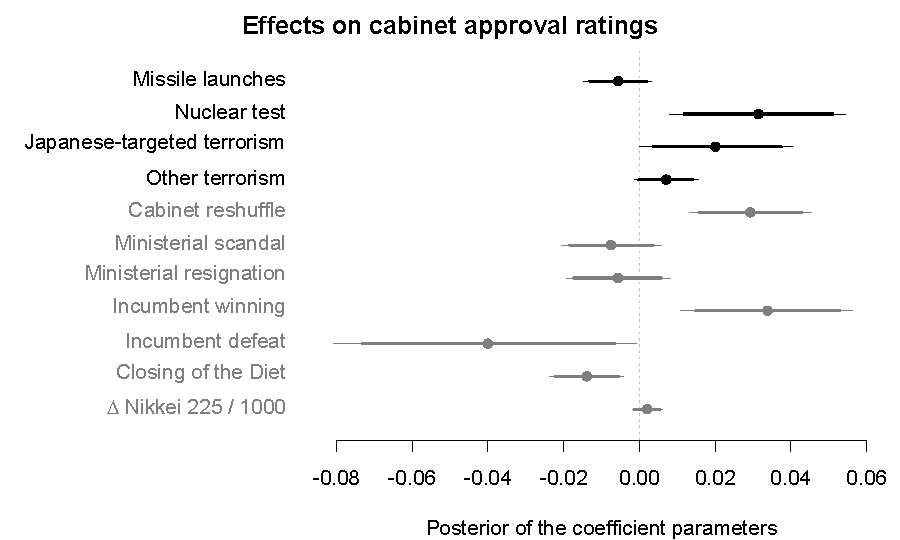
\includegraphics[scale=1]{Figure_JCR/average_effect_on_cabinet_approval.pdf}
\fi
\caption{Average Effects of Military Threat, Terrorism, and Other Control Variables on Cabinet Approval Ratings}
\label{average_effect_on_cabinet_approval}
\end{minipage}
\begin{minipage}{\hsize}
\singlespacing
\small
\emph{Notes}: Dots represent point estimates, and thick and thin lines correspond to 90\% and 95\% CIs, respectively.
\end{minipage}
\end{figure}

\section*{Additional Analysis on How Short-Lived the Effects Are}

To underscore the indispensability of the fine-grained data to detect the rally effects, we demonstrate the results of the additional analysis on how fast the effects become undetectable. We take advantage of the fact that all the polls utilized in this study were conducted at weekends, which enables us to estimate how long the rally effect continues at a daily level by interacting events with the date on which they occurred. We alter Equation~\eqref{transition_model} as follows:
\begin{equation}
\alpha _{t}=\psi + \phi \alpha _{t-1}+(t-1)\beta +\bm{\kappa}'\bm{x}_{t}+\bm{\lambda}'\bm{z}_{t}+\bm{\eta}'\bm{w}_{t}+\upsilon _{t},\label{transition_model_2}
\end{equation}

\noindent where $\bm{z}_{t}$ is a vector of the interval between the event and the poll; that is, $z_{t}=0$ if the military threats or terrorism event occurs on Friday, $z=1$ if on Thursday, $\ldots $, $z=6$ if on Saturday in the previous week. When no events happen in week~$t$, $z_{t}$ takes 0. Therefore, $\bm{\lambda}$  represents a vector of coefficients for interaction terms between events and their temporal proximity to opinion polls. If a specific event type elevates Cabinet approval ratings but its impact is short-lived, the interaction term's coefficient should be negative. Moreover, when calculating the marginal effect of events for each day of the week, it should be positive only if the events are proximal to weekends.

The results indicate that the coefficients of our main explanatory variables include zero in their 95\% CIs.\footnote{We report a detailed coefficient table for this analysis in Appendix~\ref{app:sec:misc_cabinet}.} Nonetheless, the coefficient of the interaction term between Japanese-targeted terrorism and temporal distance appears to be negative with some certainty with the posterior probability 0.961.

To interpret this, we compute the effect of Japanese-targeted terrorism on Cabinet approval ratings as a function of the day of the week on which the incident occurs. The right panel of Figure~\ref{effect_on_cabinet_approval_by_day} presents the results, with dots representing the point estimates and lines representing 95\% CIs. Shaded histograms show the distribution of the days of the week on which events occurred; the occurrence of Japanese-targeted terrorism on every day of the week suggests that the results do not heavily rely on interpolation or extrapolation. Although the even 90\% CI of the interaction term includes zero for nuclear tests, we draw the same figure also for nuclear tests in the left panel, as they are found to yield strong rally effects in our main analysis.

The right panel indicates that the 95\% CIs of the point estimates cover zero for the events happening on Saturday to Monday. Terrorist attacks that directly impact Japanese citizens lead to an increase in Cabinet approval ratings with high certainty only if the incidents occur on Tuesday or later in the week. Our results indicate that while such terrorist attacks affect citizens' opinions and induce intense rally effects, their influence attenuates quickly over three to four days. This suggests that existing studies may have failed to capture the effect due to the infrequency of polling data and the effect's short duration.

\begin{figure}[!t]
\begin{minipage}{\hsize}
\centering
\singlespacing
\if\counting0
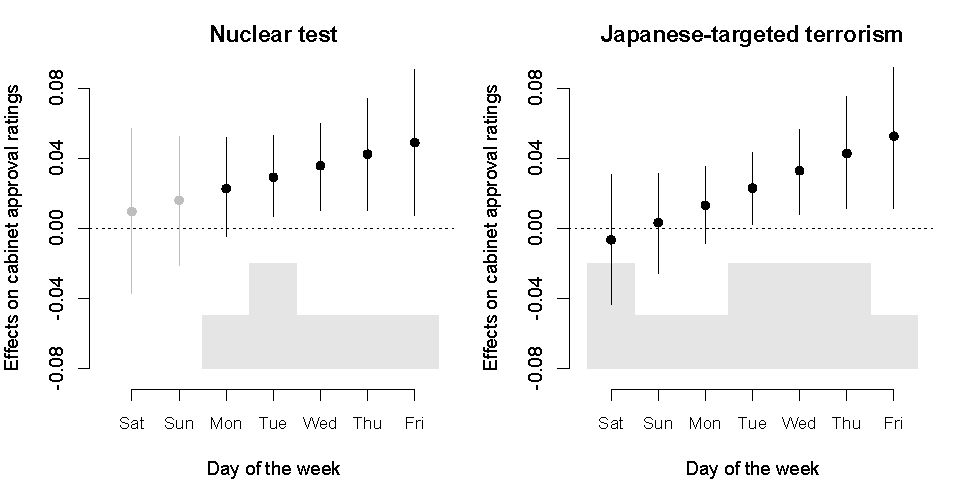
\includegraphics[scale=1]{Figure_JCR/effect_on_cabinet_approval_by_day.pdf}
\fi
\caption{Effect of Japanese-Target Terrorism on Cabinet Approval Ratings According to the Day of the Incident}
\label{effect_on_cabinet_approval_by_day}
\end{minipage}
\begin{minipage}{\hsize}
\singlespacing
\small
\emph{Notes}: Dots represent the point estimates and lines represent 95\% CIs. Shaded histograms show the distribution of the days of the week on which events occurred.
\bigskip
\end{minipage}
\end{figure}

Moreover, though we need to be highly cautious in interpreting this because of the high uncertainty of the coefficient estimate and the lack of observations on Saturday and Sunday, the simulation result for nuclear tests shown in the left panel gives us a similar impression to the result for Japanese-targeted terrorism. That is, the effect of nuclear tests on cabinet approval seems to fade away in several days. These results highlight the short-lived nature of the rally effects, as \citet{Mueller1970APSR} originally posited, and cast doubt on the validity of prior findings based on monthly or more coarse data.

\section*{Conclusion\centering}

This study empirically investigated the rally effect focusing on Japan, taking advantage of the country's pacifistic constitution to treat foreign threats as exogenous shocks. By combining data on opinion polls conducted on weekends between 2001 and 2023, we utilized a dynamic linear model to estimate the effects of North Korean military threats and terrorist attacks on Cabinet approval ratings. Our findings reveal heterogeneity in the magnitude and duration of the rally effects. In particular, North Korea's nuclear tests and Japanese-targeted terrorism have a positive impact on Cabinet approval ratings, whereas its missile launches and other terrorism do not. We also found that the effect of Japanese-targeted terrorism attenuates quickly within a week, while the effect of nuclear tests does not, highlighting heterogeneity regarding the duration of the effect.

There are several potential extensions of this study. First, it is important to directly test the mechanisms triggering the variation in the rally effect. Although we find heterogeneity across events and heterogeneity in terms of the duration of the effect, our analysis does not identify the exact mechanism that could explain these variations. Second, extending this analysis beyond the Japanese context could help generalize our findings. Third, our methodological framework can be extended to studying the effect of other types of events on government popularity. While we focused on the effects of foreign incidents, it is also worthwhile to study the effects of domestic crises that some scholars have called the rally, such as the spread of an unprecedented infectious disease \citep[e.g.,][]{Kritzinger2021WestEurPolit,Yam2020PNAS}, considering that the underlying mechanisms may be similar. Moreover, some scholars have investigated the effects of protests on public opinion, but their heterogeneity in duration, depending on the various characteristics of protests, is understudied \citep{wallace2014,jimenez-sanchez2022}. Research on these extensions may benefit from fine-grained polling data to examine the duration of the effect, especially when it is presumed that the effect would diminish quickly.

\clearpage
\bibliographystyle{apsr2}
\bibliography{bib_rally_round_the_flag,Rally}
\end{document}